%%%%%%%%%%%%%%%%%%%%%%%%%%%%%%%%%%%%%%%%%%%%%%%%%%%%%%%%%%%%%%%%%
% Tese de Doutorado / Dept. Fisica, CFM, UFSC                   %
% Lacerda@CórregoGrande - Jan/2018                              %
%%%%%%%%%%%%%%%%%%%%%%%%%%%%%%%%%%%%%%%%%%%%%%%%%%%%%%%%%%%%%%%%%

%:::::::::::::::::::::::::::::::::::::::::::::::::::::::::::::::%
%                                                               %
%                          Capítulo 3                           %
%                                                               %
%:::::::::::::::::::::::::::::::::::::::::::::::::::::::::::::::%

%***************************************************************%
%                                                               %
%                          DIG class                            %
%                                                               %
%***************************************************************%

\chapter{Classificação}
\label{sec:DIGclass}
Nosso objetivo neste trabalho é desenvolver uma maneira de caracterizar as regiões de galáxias pelo seu regime de ionização, ou seja, separar regiões SF e DIG, diferenciar componentes do DIG e ir além, servir de legado para futuros trabalhos que possam utilizar essa classificação no estudo do comportamento de diferentes propriedades estelares sob distintas componentes do ISM. Além disso, podemos analisar o víes causado pela mistura dessas diferentes componentes nas assinaturas espectrais, resolvendo o {\em conumdrum} envolvendo a espectroscopia de uma fibra (ver Seção \ref{sec:intro:partes}).

\section{O papel de $W_{H\alpha}$ na classificação das regiões: hDIG, mDIG e SFc}
\label{sec:DIGclass:WHa}

Vários trabalhos anteriores utilizam o brilho superficial de \Ha na intenção de separar regiões SF e DIG. Por exemplo \citet{Zhang.etal.2017a} argumenta que para os dados do MaNGA \citep{Bundy.etal.2015}, {\em spaxels} onde $\Sigma_{\Ha} > \Sigma_{\Ha}^{\rm SF,min} = 10^{39}$ erg$\,$s$^{-1}\,$kpc$^{-2}$ são confiavelmente dominados por SF.

Como dissemos anteriormente, nós preferimos classificar as regiões em SF e DIG baseados em $W_{\Ha}$. Vemos na classificação utilizando $\Sigma_{\Ha}$ um erro conceitual que pode ser explicado com um pequeno experimento teórico.

Imagine dois elementos de volume dominados por DIG, ambos com área superficial $A$ emitindo um fluxo $F_{\Ha}=A\times\Sigma_{\Ha}$, como na Figura \ref{fig:DIGDIG}. Assuma que o meio é opticamente translúcido para os fótons de \Ha (não há extinção), como é apropriado para regiões de DIG, de maneira que o volume inteiro seja visto. Obviamente uma operação de soma com duas regiões DIG não deve alterar a natureza da região observada. Quando na linha de visada vemos uma região ao lado da outra, medimos o mesmo brilho superficial, pois temos duas vezes o mesmo fluxo e duas vezes a mesma área, $\Sigma_{\Ha}=(2 \times F_{\Ha})/(2 \times A)$, mantendo uma classificação por um limite no brilho superfical correta. Por outro lado, quando vemos os dois elementos sobrepostos (ambos sobre a mesma linha de visada) medimos o dobro do brilho superficial, $\Sigma_{\Ha}=(2 \times F_{\Ha})/A$, fazendo com que uma operação DIG+DIG possa resultar em SF, conceitualmente errada.
%Esse viés é conceitualmente errado, pois duas regiões DIG sobrepostas deveriam continuar sendo classificadas como DIG.
Uma classificação utilizando $W_{\Ha}$ não carrega essa inconsistência por construção pois a largura equivalente final é a mesma independente da forma que os elementos são vistos.

Como veremos na Seção \ref{sec:DIGdisc:compare}, nos bojos de galáxias, onde há um percurso óptico maior, essa diferença nos critérios de classificação tem particular importância, podendo levar $\Sigma_{\Ha} > \Sigma_{\Ha}^{\rm SF,min}$ mesmo em absência de formação estelar.

De forma independente, podemos argumentar também que propriedades que possuam uma dependência radial, como cor, densidade de massa estelar, quantidade de gás, entre outras, fazem com que uma classificação usando um limite constante não seja apropriada para todas as partes de uma galáxia. Particulamente, quando o regime de ionização do DIG é orquestrado por HOLMES a disponibilidade específica de fótons que podem ionizar \Ha é basicamente constante, gerando $W_{\Ha} \sim 1\AA$ independentemente dos fluxos envolvidos (\citealt{Binette.etal.1994a}; \citealt{CidFernandes.etal.2011a}; \citealt{Belfiore.etal.2016}; ver também a Seção \ref{sec:more:kSFR}). Dessa forma é fácil entender que possam existir regiões DIG ionizadas por HOLMES (hDIG) com \Ha muito brilhante erroneamente classificadas como SF quando o parâmetro é um limite constante em $\Sigma_{\Ha}$. Da mesma forma podemos ter regiões SF fracas classificadas como DIG devido a um baixo $\Sigma_{\Ha}$.

{\ATR \ojo should I write an extensive-intensive note?} %Usando a termodinâmica como analogia, em ambos os argumentos anteriores, é a natureza extensiva de $\Sigma_{\Ha}$ que faz com haja a propensão para classificação errada entre DIG e SF. $W_{\Ha}$, por outro lado, se comporta como uma grandeza intensiva. Em termodinâmica, propriedades intensivas são aquelas que dependem


\section{A distribuição observada de $W_{H\alpha}$ e a componene hDIG}
\label{sec:DIGclass:observed}

%---------------------------- Figure ----------------------------
\begin{figure*}
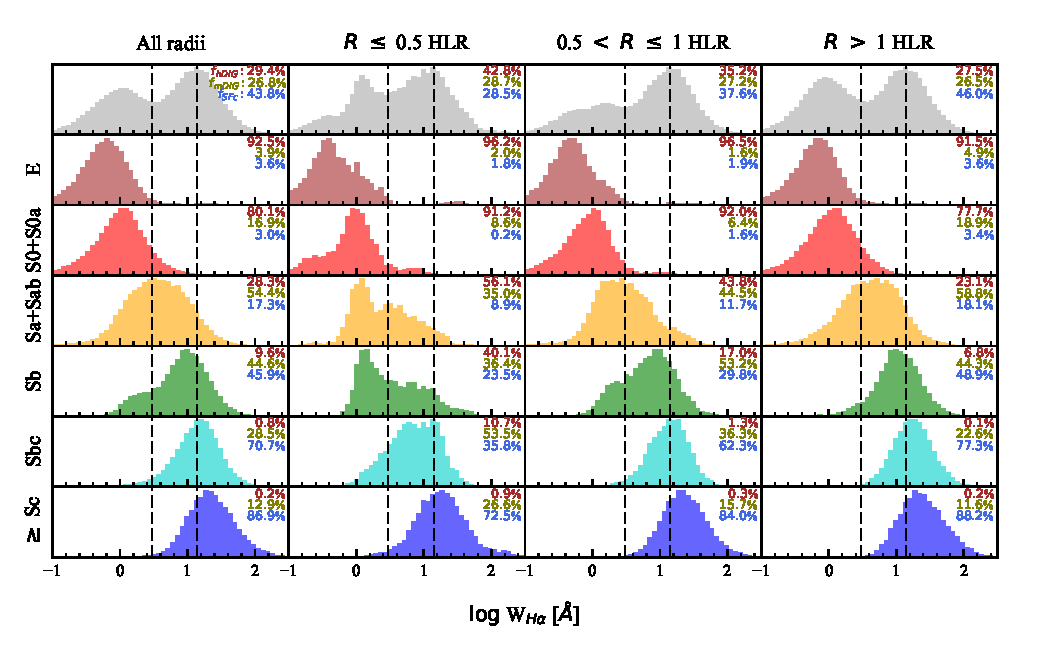
\includegraphics[scale=0.9]{figuras/fig_WHa_histograms_per_morftype_and_radius_cumulFHa.pdf}
\caption{Distribuição de $W_{\Ha}$ entre $307\,958$ zonas de 391 galáxias do CALIFA. A amostra está segmentada pela classificação de Hubble, de elípticas (segunda linha) até Sc ou mais tardias (última linha). Resultados para a amostra completa estão na primeira linha. Histogramas na primeira coluna identificam todas as regiões das galáxias. Demais colunas selecionam diferentes intervalos em raio: os primeiros 0.5 HLR internos (segunda coluna), $R = 0.5$--1 HLR (terceira) e regiões exteriores com $R > 1$ HLR (quarta). Linhas tracejadas verticais marcam 3 e 14 \AA\,, as divisões entre hDIG/mDIG e mDIG/SFc respectivamente. Os números em cada gráfico representam a fração do fluxo de \Ha associada a cada componente (valor médio entre as galáxias em cada painel).}
 \label{fig:WHaDistrib_ALLgals}
\end{figure*}
%---------------------------- Figure ----------------------------

A Figura \ref{fig:WHaDistrib_ALLgals} mostra a distribução observada de $W_{\Ha}$ para $\sim$ 300 mil zonas de 391 galáxias. Na primeira linha temos a amostra inteira e nas linhas seguintes classificamos as zonas conforme a morfologia da galáxia de onde a zona pertence; (6 classes morfológicas: E, S0-S0a, Sa-Sab, Sb, Sbc e $\ge$ Sc). Na primeira coluna temos dados de todas as regiões das galáxias, nas demais colunas classificamos as zonas por intervalos de diferentes raios: $R$ $\le$ 0.5 HLR, 0.5 < $R$ $\le$ 1 HLR, $R$ > 1 HLR.

Podemos ver que o histograma para todas as regiões de todas as galáxias (topo esquerdo) é claramente bimodal. Podemos distinguir duas populações com picos em $\sim 1 \AA$ (baixo $W_{\Ha}$) e $\sim 14 \AA$ (alto $W_{\Ha}$). Esse comportamento já foi verificado utilizando dados de galáxias do \SDSS \citep{Bamford.etal.2008a, CidFernandes.etal.2011a}. Trabalhos anteriores com dados espacialmente resolvidos do CALIFA \citep{Morisset.etal.2016} e do MaNGA \citep{Belfiore.etal.2016, Belfiore.etal.2017} também identificaram essa bimodalidade.

Estudamos também os mesmos histogramas sem a binagem espacial (todos os {\em spaxels}) e, apesar da alteração na amplitude relativa entre os dois picos, a bimodalidade se mantém e dois fits gaussianos do histograma para todos os dados continua identificando duas componentes, com centros em $\sim 1$ e $14 \AA$.

Nós interpretamos essa população com baixas larguras equivalentes como regiões DIG fotoionizadas por HOLMES. Como teste, podemos calcular $\xi$, a razão entre a luminosidade de \Ha observada e aquela esperada pelos fótons produzidos pelas populações mais velhas que $10^8$ anos através da análise com o \starlight, seguindo a metodologia aplicada em \citet{CidFernandes.etal.2011a}. Como os modelos de populações estelares utilizados pela síntese \citep{Gonzalezdelgado2005, Vazdekis2010} não possuem a parte ionizante nos espectros ($h\nu > 13.6$ eV) tomamos emprestado aqueles de \citet{Bruzual.Charlot.2003} utilizando uma função inicial de massa ({\em initial mass function}; IMF) de Salpeter e as trilhas estelares de \citet{Girardi2000}. Como discutido em \citet{CidFernandes.etal.2011a} diferentes modelos produzem diferenças sistematicas de 0.2--0.5 dex na quantidade  prevista de fótos ionizantes. A Figura \ref{fig:WHa-Xi} mostra $\xi$ em função de $W_{\Ha}$, com os histogramas coloridos por nossa classificação hDIG/mDIG/SFc. Encontramos que $\xi$ é de ordem 1 para as regiões com baixo $W_{\Ha}$. Consequentemente, apesar de todas as incertezas envolvidas nesse cálculo \citep{CidFernandes.etal.2011a, Belfiore.etal.2016, Morisset.etal.2016}, o resultado final corrobora a interpretação de que HOLMES são responsáveis pela população de baixo $W_{\Ha}$.

% Seja $L_{\Ha}$ a luminosidade observada de \Ha e $L_{\Ha}^{\rm exp}(t > 10^8 {\rm anos})$ a luminosidade esperada pelas populações velhas, definimos a razão como:
% \begin{equation}
%   \xi\ =\ \frac{L_{\Ha}}{L_{\Ha}^{\rm exp}(t > 10^8 {\rm anos})}.
% \end{equation}
% \noindent Podemos definir

%---------------------------- Figure ----------------------------
\begin{figure}
 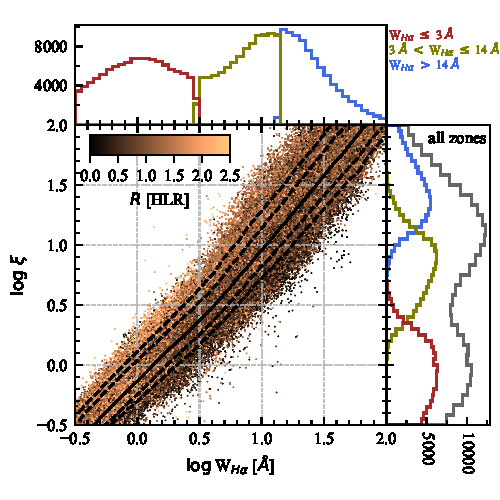
\includegraphics[scale=1.5]{figuras/fig_logxi_logWHa_histograms.pdf}
 \caption{Razão entre a luminosidade de \Ha observada e aquela predita pelas poulações mais velhas que $10^8$ anos ($\xi$) em função de $W_{\Ha}$ para todas as zonas de nossa amostra. Os pontos estão coloridos conforme a distânciada até o núcleo (em unidades de HLR). Os histogramas de $\xi$ e de $W_{\Ha}$ estão coloridos como vermelho/amarelo/azul (hDIG/mDIG/SFc), mostrando que as regiões com baixo $W_{\Ha}$ são compatíveis com ionização por HOLMES.}
 \label{fig:WHa-Xi}
\end{figure}
%---------------------------- Figure ----------------------------

Fica evidente a correspondência dessa interpretação com o conceito de galáxias aposentadas apresentado por \citet{Stasinska.etal.2008a}. Estes são sistemas que pararam de formar estrelas há muito tempo e os fótons presentes são provenientes das estrelas que já evoluíram após o ramo assintótico das gigantes ({\em post-asymptotic giant branch; post-AGB}) e anãs brancas levando os valores de $W_{\Ha}$ a $\sim 1$ \AA. O limite de 3 \AA\ coincide com o valor utilizado por \citet{CidFernandes.etal.2011a} para distinguir galáxias aposentadas daquelas com regime de ionização dominado por SF ou por AGN. Por esse motivo nós afirmamos que as populações com $W_{\Ha} < 3$ \AA\ sejam classificadas como gás difuso ionizado por HOLMES, o hDIG.

A segmentação da distribuição de $W_{\Ha}$ pelos tipos de Hubble mostra que a bimodalidade está sempre presente, mudando apenas a proporção entre as populações de baixo e alto $W_{\Ha}$ conforme a morfologia: galáxias {\em early-type} são esmagadoramente dominadas por valores ao redor do pico de $\sim 1$ \AA, enquanto nas galáxias espirais tardias é a população com alto $W_{\Ha}$ que domina.

Quando dividimos a amostra em intervalos de $R$ vemos que a população hDIG se distribui igualmente nas galáxias {\em early-type}, confirmando estudos anteriores de \citet{Kehrig.etal.2012}, \citet{Singh.etal.2013}, e \citet{Gomes.etal.2016b}, além das análises baseadas em dados do MaNGA por \citet{Belfiore.etal.2016, Belfiore.etal.2017}. Entre as Sb e espirais mais tardias o hDIG fica concentrado nas regiões centrais das galáxias. Para colocar isso em números, 82\% dos pontos hDIG das 225 galáxias Sb ou mais tardias estão localizados em regiões onde $R < 1$ HLR.

%% End of this chapter
